\documentclass[12pt]{article}
\usepackage{ctex}
\usepackage[english]{babel}
\usepackage[utf8x]{inputenc}
\usepackage{amsmath}
\usepackage{graphicx}
\usepackage[colorinlistoftodos]{todonotes}
\usepackage{multirow}
\usepackage{subfigure}
\usepackage{lineno}
\usepackage{amsfonts}              % for blackboard bold, etc
\usepackage{amsthm}       
\usepackage{booktabs}
\usepackage{apacite}
\usepackage{caption}
\usepackage{graphicx, subfig}
\usepackage{subfigure}

% 这是为了显示中文字体
\usepackage[UTF8]{ctex}

%\linenumbers
%\usepackage[singlelinecheck=false]{caption} %for left aligned captions

\setlength{\evensidemargin}{0in}
\setlength{\oddsidemargin}{0in}
\setlength{\topmargin}{0in}
\setlength{\textwidth}{6.25in}
\setlength{\parindent}{0cm}
\setlength{\textheight}{9in}
%\setlength{\parskip}{1ex}
\setlength{\baselineskip}{22pt}
\setlength{\topsep}{1ex}

\usepackage{soul}
\usepackage[top = 2cm, bottom = 2cm, left = 3cm, right =2cm]{geometry}


\begin{document}

\begin{titlepage}

\newcommand{\HRule}{\rule{\linewidth}{0.5mm}} % Defines a new command for the horizontal lines, change thickness here

\center % Center everything on the page

\textsc{\LARGE Tongji University}\\[1.5cm]
\textsc{\Large School of Software Engineering}\\[0.5cm]
\textsc{\large GAN+RL For Anomaly Detection}\\[0.5cm]

\HRule \\[0.4cm]
{ \huge \bfseries X-Lab Report}\\[0.4cm] % Title of the report
\HRule \\[1.5cm]

\begin{minipage}{0.5\textwidth}
\begin{flushleft} \large
\emph{\textbf{Student:}}\\
Name: Liang \textsc{Wang} \\
E-mail: leonwangchn@163.com \\
\end{flushleft}
\end{minipage}
~
\begin{minipage}{0.4\textwidth}
\begin{flushright} \large
\emph{Instructor:} \\
Jasper \textsc{Qiu}
\end{flushright}
\end{minipage}\\[2cm]


{\large \today}\\[2cm]


\vfill % Fill the rest of the page with whitespace

\end{titlepage}

\tableofcontents


\newpage

\section{Report 1}

\subsection{\textbf{Introduction}}
异常检测的特点:

1. 单变量时序分类问题 \\
2. 异常数据占的比例很小(样本不均衡)  => 传统分类方法不适用 \\
3. 异常的三种类型:contextual anomaly, point anomaly, collective anomaly \\
4. 异常都有 global 和 local 两种模式,其中 local 和正常数据有相同的分布,所以更难识别  => 普通的深度学习模型不适用 \\

Contributions:\\
1. 设计了用于异常检测的CLSTM \\
2. 数据预处理,消除样本不均衡 \\
3. new model = CLSTM + GAN + RL \\


\subsection{\textbf{Background}}
\subsubsection{传统分类方法}
传统分类方法仅在 statistical anomalies 上表现好,但是不能准确区分与正常数据有同样分布的异常数据

\subsubsection{DL 方法}
C-LSTM
\begin{itemize}
\item 结合cnn与rnn, can both extract temporal and spacial features in data sequences
\item cnn与lstm线性连接
\item 论文6
\item 原本用于文本分类,本文重新设计后用于异常检测
\item 实际上本文中的模型和实验数据来自论文2
\end{itemize}

\subsubsection{GAN 方法}
论文1:
\begin{itemize}
\item 基于GAN进行异常检测

\item background倒数第二段提到其缺点:不能处理时序数据
\end{itemize}
论文3:
\begin{itemize}
\item 能处理时序数据的GAN:SeqGAN

\item 但是是用于生成word sentences的,其数据特征与异常检测不同(离散与连续),所以不能应用于异常检测

\item 但可以借鉴其部分思想,即引入强化学习
\end{itemize}
\subsubsection{综上}
综上:有多种方法能够实现对数据序列的异常检测。一是CSTM,可以提取时空特征。二是GAN,更能够很好地学到数据的值的分布。所以本文模型结合以上两种网络:

CNN + RNN + GAN + RL

\subsection{\textbf{Our Model}}
CNN + LSTM => 分类器

GAN + RL => 解决数据不平衡问题

\begin{figure}[htbp]

\centering

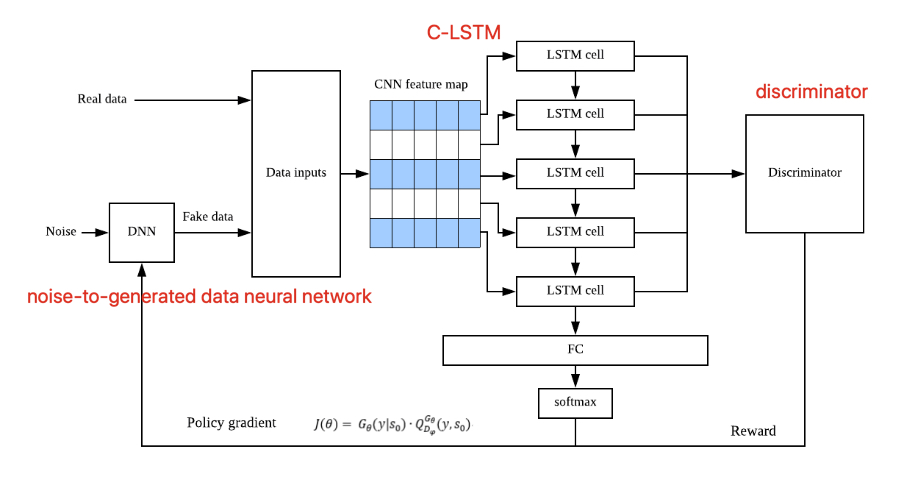
\includegraphics[height=9cm,width=14.25cm]{network.jpg}

\caption{Network}

\end{figure}

\subsubsection{C-LSTM Classifier for AD}
介绍用于异常检测的C-LSTM网络,取自论文2

\subsubsection{GAN for AD}
正样本太少,所以传统深度学习模型不好

介绍最早用于异常检测的GAN,即论文1中的模型

借鉴论文3中的思想,构建 SeqGAN 模型,引入强化学习

\subsubsection{GAN via Policy Gradient}
SeqGAN 中的策略梯度算法,借鉴论文3

用GAN解决数据不平衡问题,在引入seqGAN解决提取时空特征的问题,再把GAN与RL结合,解决只能用于离散数据的问题

不需要使用蒙特卡洛搜索dual


\subsubsection{Training}
具体训练的过程,在论文3的基础上进行的修改

训练的过程:

1. 先预训练CLSTM分类器。只用不含异常的sequence进行训练,所以此时它并不能很好地区分无异常sequence和有异常sequence,但是它能很好地区分真实数据和生成的数据。 \\
2. 训练生成数据的网络 \\
3. 训练判别器网络 \\
4. 重复2~3,进行对抗


\subsubsection{Anomaly Assessment}
对于DL方法:直接评估序列是否异常

对于GAN+RL方法:

\begin{itemize}
\item 针对single data,而不是sequence
\item 通过判别器的一些中间层的输出计算一个分数,从而判定是否异常
\end{itemize}

\subsection{\textbf{Experiment}}
\subsubsection{Yahoo S5 数据集和数据预处理}

滑窗算法进行预处理,把 single data 处理成 sequence,正样本比例 1669/94866 => 8556/90913 

\subsubsection{软硬件}

\subsubsection{DL 方法的实验}
(这部分完全来自论文2,可能只是为了和4.4的实验做个对比,没有太大的意义)

最终的结论是 CNN + LSTM + DNN 的网络结构比其他 DL 网络表现更好

\subsubsection{GAN 方法的实验}
以论文1中的 GAN 模型作为 benchmark,实验证明我们提出的 GAN + RL 模型表现更好

\newpage
\subsection{\textbf{引文研究}}

\subsubsection{CLSTM相关}\label{header-n516}

\textbf{{[}6{]}Chunting Zhou, Chonglin Sun, ''A C-LSTM Neural Network
for Text Classification'', November 2015.}

提出了C-LSTM,结合CNN和LSTM,提取空间和时间特征,用于文本分类。

本文进行重新设计后,用于异常检测。

\begin{quote}
C-LSTM(proposed by Chunting Zhou, Chonglin Sun, 2015{[}?{]}) is to make
use of the two features. It consists of CNN and LSTM layers, structured
linearly. The spatial features of the data sequence is extracted by the
convolution and pooling layers, and the temporal features are extracted
by the LSTM layers. C-LSTM was proposed to do text classification, we
redesigned the network structure and use it to do anomaly detection.
\end{quote}

\textbf{{[}2{]}Tae-Young Kim, Sung-Bae Cho, ''Web traffic anomaly
detection using CLSTM neural networks'', Expert Systems With
Applications 106 (2018) 6676, 2018}

SCI 期刊

摘要

Web traffic refers to the amount of data that is sent and received by
people visiting online websites. Web traffic anomalies represent
abnormal changes in time series traffic, and it is important to perform
detection quickly and accurately for the efficient operation of complex
computer networks systems. In this paper, we propose a C-LSTM neural
network for effectively modeling the spatial and temporal information
contained in traffic data, which is a one-dimensional time series
signal. We also provide a method for automatically extracting robust
features of spatial-temporal information from raw data. Experiments
demonstrate that our C-LSTM method can extract more complex features by
combining a convolutional neural network (CNN), long short-term memory
(LSTM), and deep neural network (DNN). The CNN layer is used to reduce
the frequency variation in spatial information; the LSTM layer is
suitable for modeling time information; and the DNN layer is used to map
data into a more separable space. Our C-LSTM method also achieves nearly
perfect anomaly detection performance for web traffic data, even for
very similar signals that were previously considered to be very
difficult to classify. Finally, the C-LSTM method outperforms other
state-of-the-art machine learning techniques on Yahoo's well-known
Webscope S5 dataset, achieving an overall accuracy of \textbf{98.6\%}
and recall of \textbf{89.7\%} on the test dataset. (C) 2018 Elsevier
Ltd. All rights reserved.

论文中 deep learning experiments 中的数据来自此文。

CLSTM应用于异常检测,CNN + LSTM + DNN 的表现最好。

\subsubsection{GAN相关}\label{header-n520}

\textbf{{[}1{]}Houssam Zenati, Chuan-Sheng Foo, ''Efficient GAN-Based
Anomaly Detection'', Workshop Track, ICLR, 2018}

\begin{itemize}
\item
  提出了把 GAN 应用于异常检测。生成器和判别器都采用 DNN
  结构,并通过计算测试样本和生成样本的距离作为异常评估。缺点是指处理没有时间的数据。

  提供了 GAN 的思路,提供了通过计算距离进行异常评估的思路。

  discriminator
  不只考虑输入(真实还是生成的),还考虑输入的潜在表示,从而进行分类
\end{itemize}

\begin{itemize}
\item
  在 GAN 实验中被用作benchmark

  \begin{quote}
  we constructed experiments on our GAN model. We use another GAN
  network (Houssam Zenati {[}?{]}) which simply uses DNN network in
  generator and discriminator as benchmark. This model is designed to do
  anomaly detection in KDD dataset, and this data set is not
  time-serial, that is, neighboring data is independent with each other.
  So the benchmark model doesn't using the spatial and temporal
  information, and when updating parameters via gradients, this model is
  quite traditional, while our model using policy gradient.
  \end{quote}
\end{itemize}

\textbf{{[}3{]}Lantao Yu, Weinan Zhang, ''SeqGAN: Sequence Generative
Adversarial Nets with Policy Gradient'', AAAI, 2017 }

在论文{[}1{]}的基础上,提出能够处理时间序列的 GAN(通过LSTM),即
SeqGAN。

缺点是它处理的数据的值是离散的,而异常处理数据的值是连续的,所以不能直接用于异常处理。但可以借鉴其中的思想,如引入
RL。

\subsubsection{其他}\label{header-n191}

\textbf{{[}4{]}Bachman, P., and Precup, D., ''Data generation as
sequential decision making'', NIPS, 32493257, 2015i}

SeqGAN 的引文

sequential procedures for generating data
指的是生成模型,强化学习对此提供帮助

MDP:马尔可夫决策过程

生成模型的训练 与 强化学习中的策略搜索 相结合

结合 data imputation(数据填补/缺失值处理)问题进行讨论

\textbf{{[}5{]}Bengio, S.; Vinyals, O.; Jaitly, N.; and Shazeer,N.,
''Scheduled sampling for sequence prediction with recur-rent neural
networks'', NIPS, 11711179, 2015}

SeqGAN 的引文

提出了训练 RNN 的 trick:计划采样

scheduled sampling翻译成``计划采样'', 用于解决exposure bias问题
针对sequence-to-sequence框架下的decoder阶段,在训练时,生成\(y_{t}\)时,输入的\(y_{t-1}\)是训练集中标注序列中的true
value, 然后在预测是,输入的\(y_{t-1}^{\prime}\)是在t-1时刻生成的label,
该标签可能是正确的,也可能是预测错误的标签,如果是错误的标签就会导致一个问题,就是错误爆炸,说白了就是\(y_{t-1}^{\prime}\)是错误标签,那么以它为输入生成的\(y_{t}\)也是不可信的。针对这种问题,提出了scheduled
sampling的解决方法。 Scheduled
Sampling是指RNN训练时时会随机使用模型真实label来作为下一个时刻的输入,而不像原先那样只会使用预测输出。
训练时网络将不再完全采用真实序列标记做为下一步的输入,而是以一个概率p选择真实标记,以1-p选择模型自身的输出。``计划采样''即p的大小在训练过程中是变化的,就像学习率一样。作者的思想是:一开始网络训练不充分,那么p尽量选大值,即尽量使用真实标记。然后随着训练的进行,模型训练越来越充分,这时p也要减小,即尽量选择模型自己的输出。这样就尽量使模型训练和预测保持一致。

\subsection{\textbf{疑问}}

\begin{enumerate}
\def\labelenumi{\arabic{enumi}.}
\item
  为什么说异常数据和正常数据可以有相同的分布?
\item
  为什么网络可以对 single data 进行异常评估
\end{enumerate}

\newpage

\section{Report 2}

研究学习了原论文的这篇引文,学习GAN用于异常检测的基本思想,并通过实验进行了验证。

\textbf{{[}1{]}Houssam Zenati, Chuan-Sheng Foo, ''Efficient GAN-Based
Anomaly Detection'', Workshop Track, ICLR, 2018}

\subsection{\textbf{摘要}}

生成式对抗网络(GANs)能够模拟真实世界数据的复杂高维分布,这表明它们可以有效地进行异常检测。然而,很少有人探索将GANs用于异常检测任务。我们利用最近开发的GAN模型进行异常检测,并且在图像和网络入侵数据集上达到了目前为止最好的表现,同时在测试时间上比目前发布的基于GAN的方法快数百倍。

\subsection{\textbf{介绍}\label{header-n3}}

异常检测是一系列领域中最重要的问题之一,包括制造业,医学影像和网络安全。\textbf{异常检测方法需要对正常数据的分布进行建模,正常数据可以是复杂的、高维的}。生成式对抗网络(GANs)是一类已经成功地用于对这种复杂的和高维分布进行建模的模型,特别是在自然图像上。

\begin{figure}[htbp]
\centering
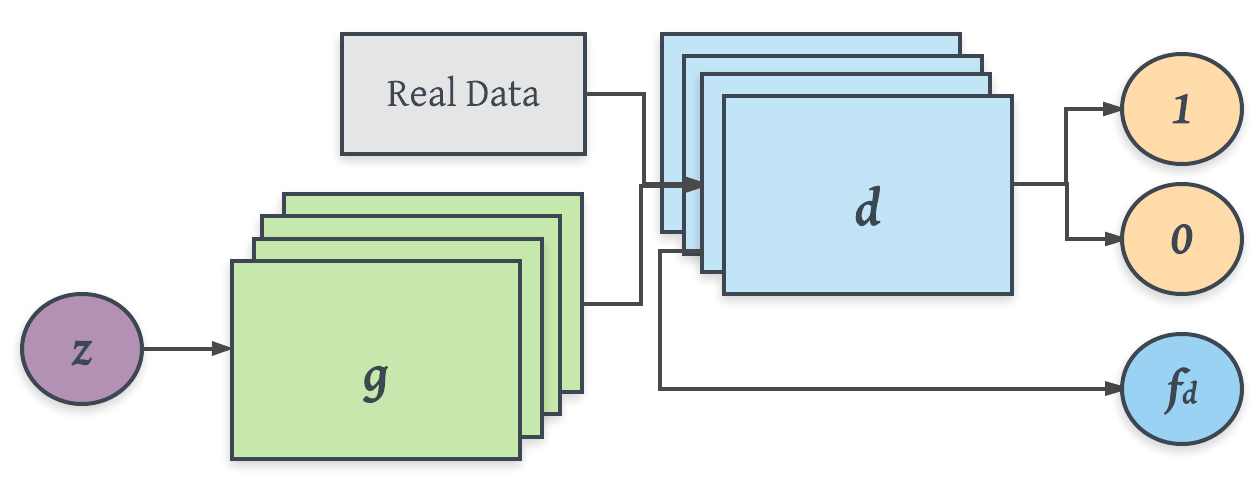
\includegraphics[height=5cm,width=12cm]{Report2-figure/gan.png}
\caption{GAN}
\end{figure}


直观地说,基于正常样本的分布进行过良好训练的GAN应该能够从一个\textbf{潜在的}表示\textbf{重建}这样的正常样本,并且还能对来自真实数据分布的样本进行\textbf{区分}。

然而,因为GANs仅隐式地对数据分布进行建模,使用它们进行异常检测需要\textbf{昂贵的优化过程}来恢复给定输入示例的潜在表示,使得这对于大型数据集或实时应用来说是\textbf{不切实际}的方法。

在这项工作中,我们利用GAN方法,同时在训练期间训练一个\textbf{编码器},以开发一种高效的异常检测方法。

我们将我们的方法应用到图像数据集MNIST,以及一个网络入侵数据集kdd99
10percent,表明它与其他方法相比具有很强的竞争力。据我们所知,我们的方法是第一种基于GAN的异常检测方法,它在kdd99数据集上实现了目前最好的结果。

\subsection{\textbf{相关工作}\label{header-n11}}

异常检测已被广泛研究,如比较流行的利用聚类方法或最近邻方法和单分类方法学习正常数据周围的判别边界,如单类SVM)。另一类方法使用重构的似然性来确定一个例子是否异常,并且包括主成分分析(PCA)及其核和鲁棒变量。最近的作品使用深度神经网络,不需要明确的特征构造,不同于前面提到的方法。自动编码器、变分自编码器、基于能量的模型和深度自编码高斯混合模型已被探索用于异常检测。然而,尽管GANs适合模拟现实世界数据的高维复杂分布,除了AnoGAN,使用GANs进行异常检测的研究还相对较少。

\subsection{\textbf{GANs 进行高效地异常检测}\label{header-n13}}

\subsubsection{训练}\label{header-n14}

\begin{figure}[htbp]
\centering
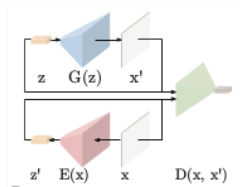
\includegraphics[height=5cm,width=8cm]{Report2-figure/image-20191001141522578.png}
\caption{BiGAN训练}
\end{figure}


\begin{figure}[htbp]
\centering
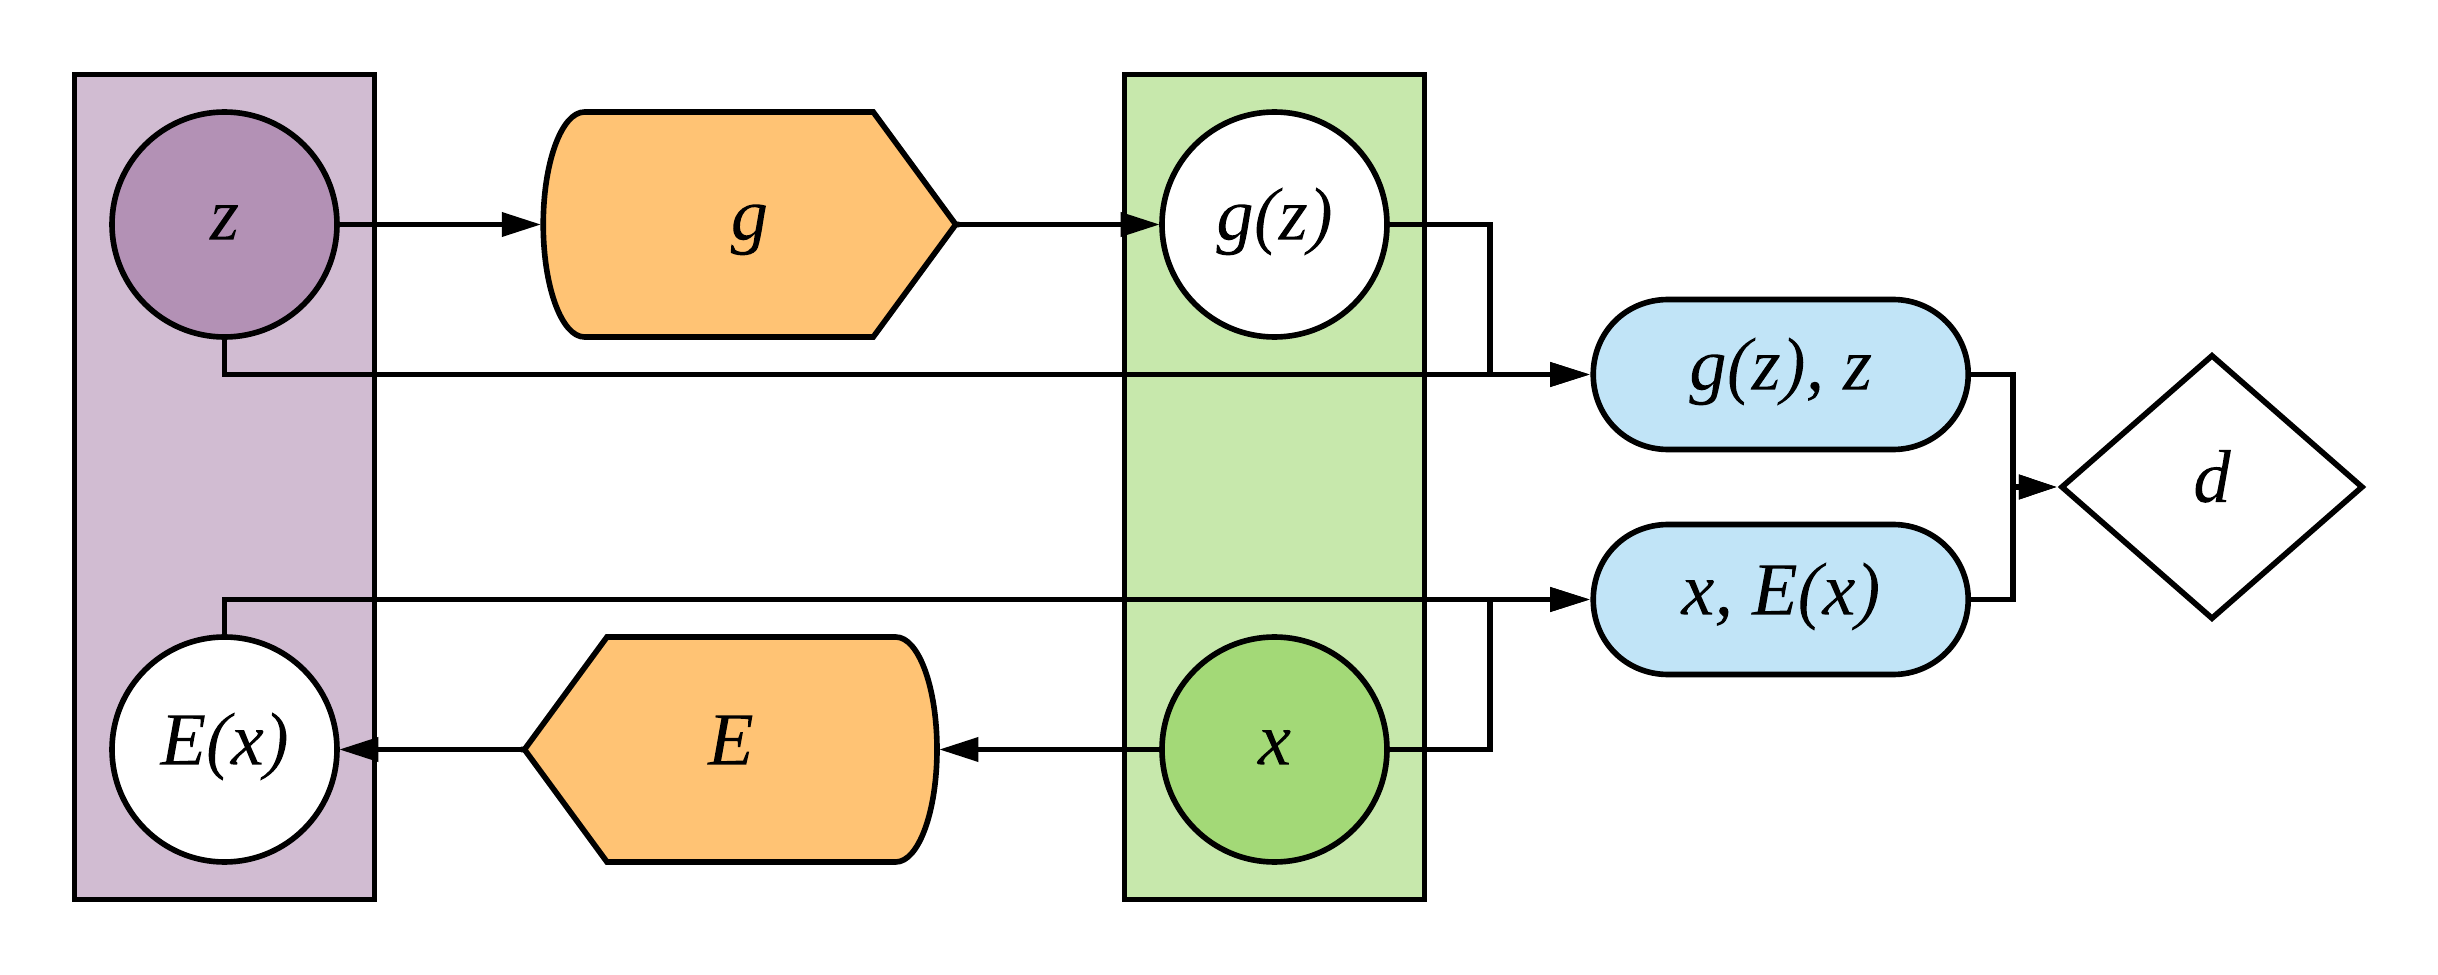
\includegraphics [height=5cm,width=12cm]{Report2-figure/bigan_train.png}
\caption{BiGAN训练}
\end{figure}

我们的模型基于BiGAN:在训练期间,除了训练生成器G和鉴别器D之外,同时学习了将输入样本x映射到潜在表示z的编码器E。这使我们能够避免在检测阶段时恢复潜在表示的计算量大的步骤。
与常规GAN中的鉴别器仅考虑输入(实际或生成)不同,鉴别器D在这种情况下还考虑了潜在表示(来自生成器的输入或来自编码器的输出)。

Vincent
Dumoulin&Courville探索了不同的训练策略来学习编码器\(E=G^{-1}\),并强调了与G一起学习E的重要性。因此,我们采用了类似的策略,在训练过程中解决了以下优化问题:\(\min _{G, E} \max _{D} V(D, E, G)\),其中\(V(D, E, G)\)定义为

\[V(D, E, G)=\mathbb{E}_{x \sim p_{X}}\left[\mathbb{E}_{z \sim p_{E}(\cdot | x)}[\log D(x, z)]\right]+\mathbb{E}_{z \sim p_{Z}}\left[\mathbb{E}_{x \sim p_{G}(\cdot | z)}[1-\log D(x, z)]\right]\]

在此,\(p_{X}(x)\)是数据的分布,\(p_{Z}(z)\)是潜在表示的分布,\(p_{E}(z | x)\)和\(p_{G}(x | z)\)分别是编码器和生成器引起的分布。

\subsubsection{推断(检测)}\label{header-n21}

\begin{figure}[htbp]
\centering
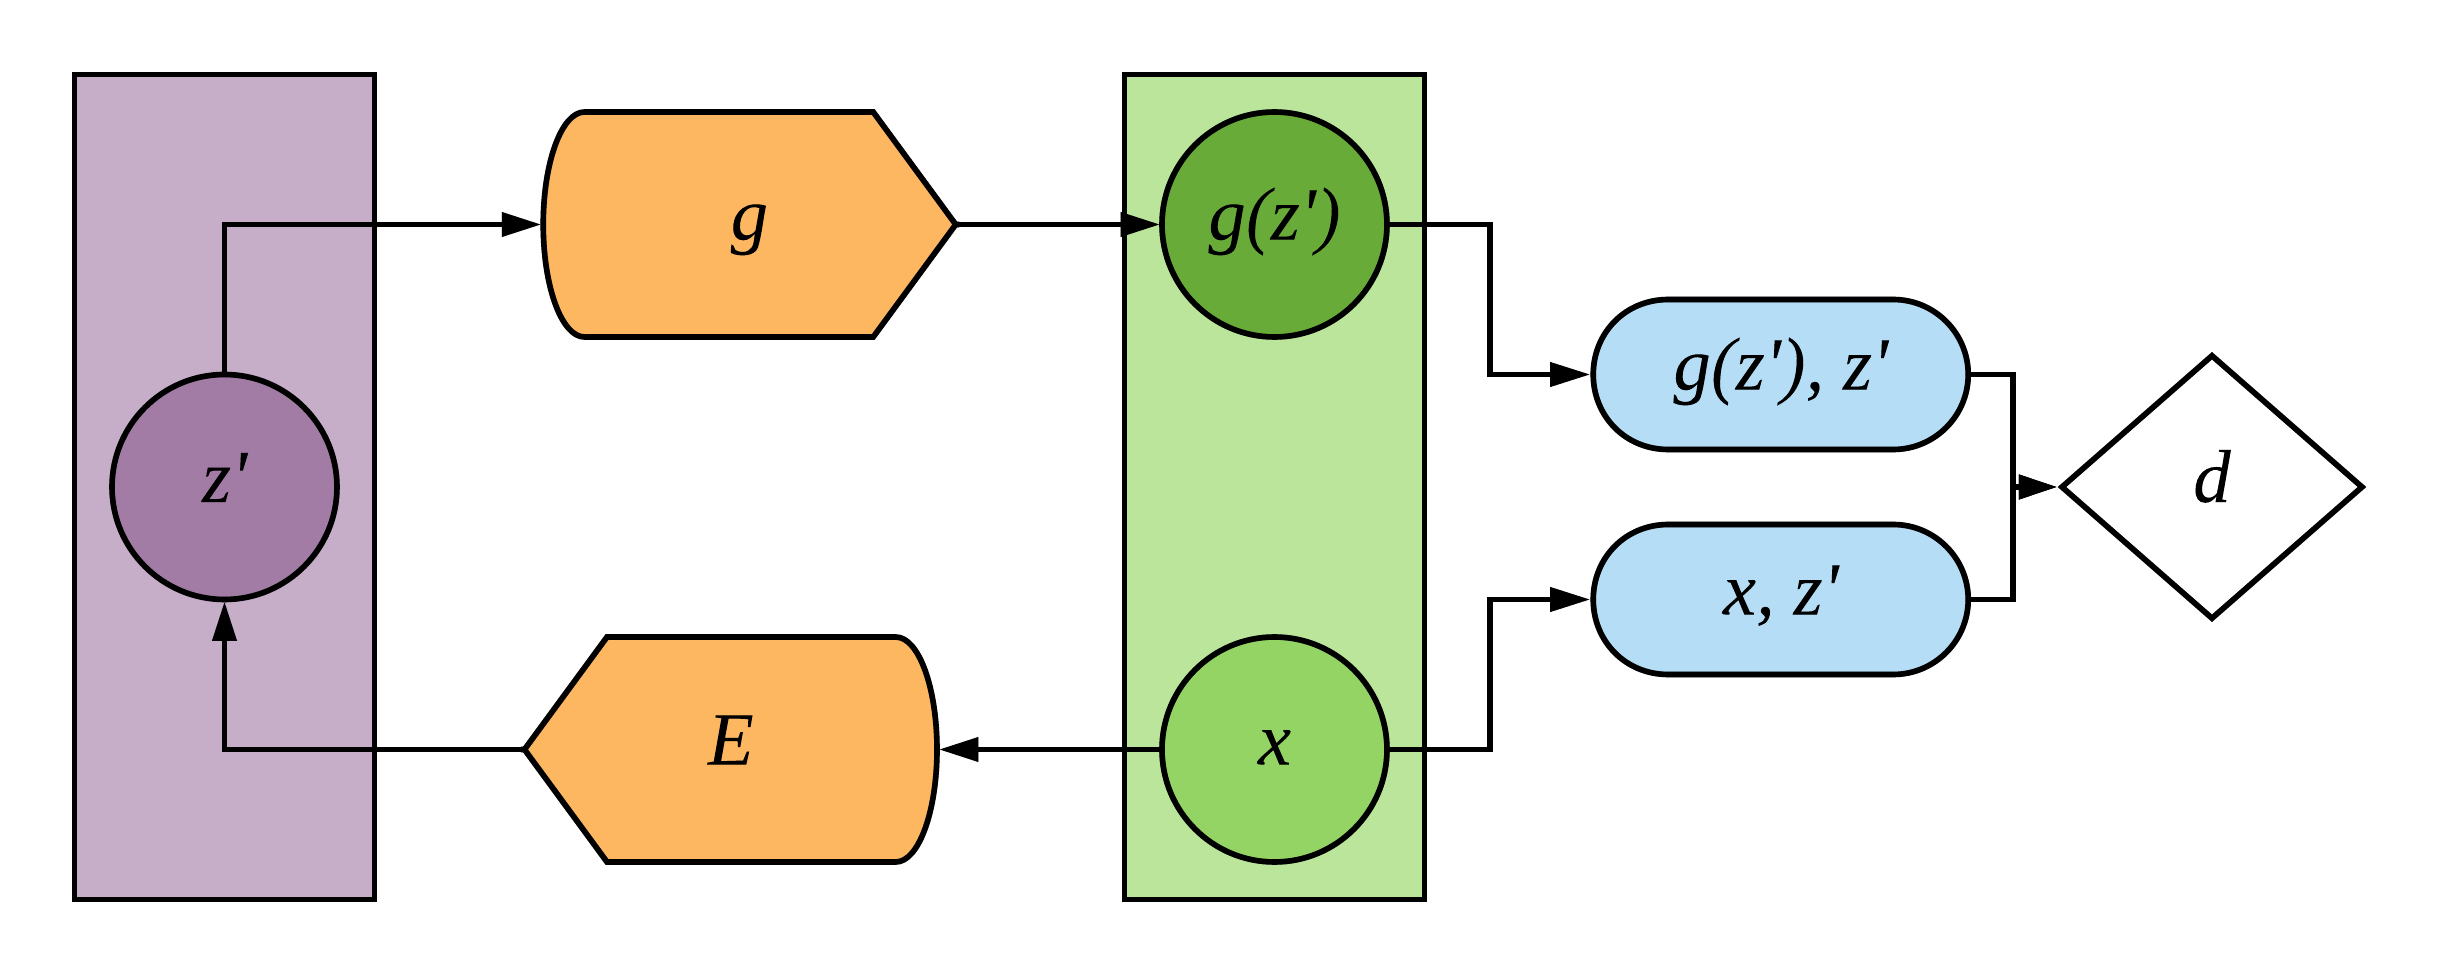
\includegraphics[height=5cm,width=12cm]{Report2-figure/image-20191001150021322.png}
\caption{BiGAN推断}
\end{figure}

在\textbf{正常数据上训练}了模型以产生G,D和E之后,我们定义了一个得分函数A(x),基于重构误差\(L_G\)和判别器误差\(L_D\)的凸组合:

\[A(x)=\alpha L_{G}(x)+(1-\alpha) L_{D}(x)\]

\begin{quote}
凸组合:一类特殊的线性组合
\end{quote}

其中\(L_{G}(x)=\|x-G(E(x))\|_{1}\)。

\(L_{D}(x)\)可以用两种方式定义

\begin{itemize}
\item
  第一种,使用鉴别器认为x是一个真实数据(1类)的交叉熵损失σ:\(L_D(x) = \sigma(D(x, E(x)), 1)\),它捕获了鉴别器A认为样本服从真实数据分布的可信度。
\item
  第二种方法是``特征匹配损耗''\(L_D(x)=\left\|f_{D}(x, E(x))-f_{D}(G(E(x)), E(x))\right\|_{1}\)
  ,其中\(f_D\)返回鉴别器中给定输入的对数之前的层。
  这可以评估重构数据在鉴别器中是否具有与真实样本相似的\textbf{特征}。 
\end{itemize}

具有较大A(x)值的样本被认为更可能是异常的。

\subsection{\textbf{实验}\label{header-n37}}

\subsubsection{MNIST}\label{header-n38}

10个数据集:分别以一个数字作为异常,剩下九个作为正常。训练集包含80\%的正常数据,测试集包含20\%正常数据和全部的异常数据。

所有模型只接受正常数据的训练,并用正常和异常数据进行测试。由于数据集是不平衡的,我们使用模型在精确召回曲线(AUPRC)下的面积进行比较。我们评估了我们的方法对比AnoGAN和变分自编码器(VAE)的效果。我们发现,我们的模型显著优于VAE基线。同样,我们的模型优于AnoGAN,但具有大约快800倍的推断时间。我们还观察到,在异常分数中\(L_D\)使用特征匹配损失比交叉熵损失更好,这表明鉴别器提取的特征为异常检测提供了信息。

\subsubsection{KDD99}\label{header-n41}

我们用这个网络活动数据集评估了我们的方法,显示GANS也可以很好地表现在高维、非图像数据。我们遵循kddcup99
10percent数据集上的实验设置。由于数据集中异常值的比例,``正常''数据在本任务中被视为异常。20\%个异常得分\(A(x)\)最高的样本被分类为异常(阳性类),并据此评价精度、召回率和F1得分。为了训练,我们随机抽样50\%的整个数据集,其余50\%的数据集被用于测试。然后,只有正常样本的数据样本被用于训练模型,因此,所有异常样本从分裂训练集中被移除。我们的方法总体上与其他最先进的方法具有很强的竞争力,并实现更高的召回率。再一次,我们的模型性能好,并且有更快的推断速度。

预处理:数据集包含41个维度的样本,其中34个样本是连续的,而7个是分类的。
对于分类特征,我们进一步使用一键表示法对其进行编码;
经过这种编码,我们总共获得了121个特征。
然后,我们应用最小-最大缩放进行特征缩放,来得出最终特征。

\subsection{\textbf{结论}\label{header-n45}}

我们证明了最新的GAN模型可用于实现对高维、复杂数据集进行异常检测的最新性能,同时在推断时效率很高。
我们使用GAN的同时学习编码器,消除了为恢复给定输入的潜在表示而使用的昂贵过程的需要。
在未来的工作中,我们计划对我们的方法进行更广泛的评估,评估其他训练策略,并探索编码器精度对异常检测性能的影响。

\subsection{\textbf{实验过程}\label{header-n87}}

代码

\begin{verbatim}
python3 main.py gan kdd run --nb_epochs=10 --label=0
\end{verbatim}

\begin{figure}[htbp]
\centering
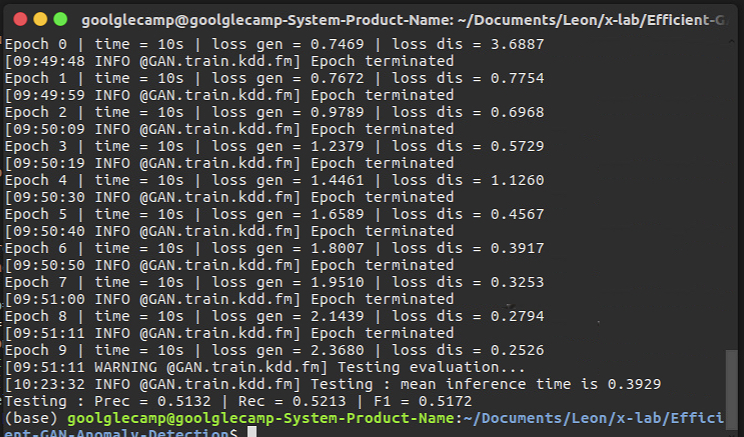
\includegraphics[height=7cm,width=12cm]{Report2-figure/image-20191001134406795.png}
\caption{GAN实验}
\end{figure}

\begin{verbatim}
python3 main.py bigan kdd run --nb_epochs=10 --label=0
\end{verbatim}

\begin{figure}[htbp]
\centering
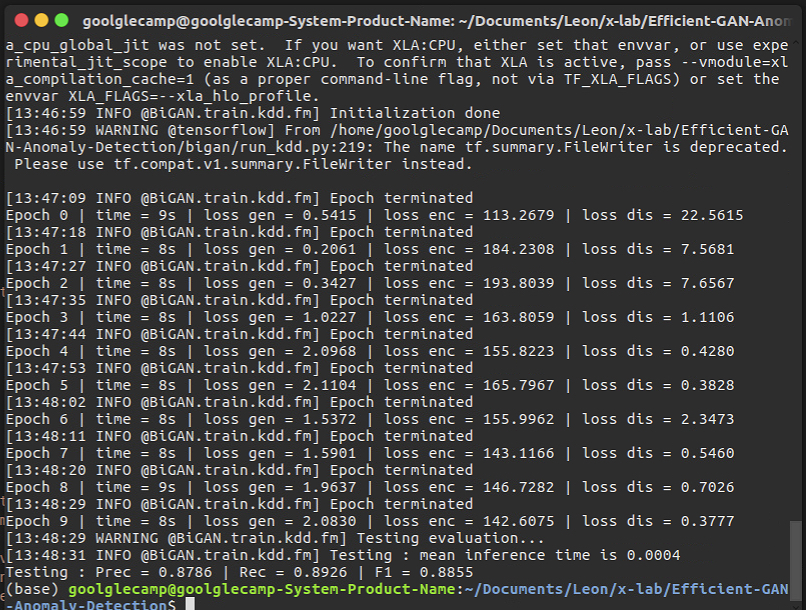
\includegraphics[height=8cm,width=12cm]{Report2-figure/image-20191001134929348.png}
\caption{BiGAN实验}
\end{figure}

\subsection{\textbf{总结}\label{header-n58}}

\subsubsection{对我们课题的意义}\label{header-n85}

提供了利用GAN进行异常检测的基本思路。训练阶段,使用正常数据训练GAN,使其学到正常数据的分布。推断阶段,设计一个评估异常得分的函数,计算样本异常的程度,设定阈值进行异常的分类。距离指的是样本在潜在特征空间中的距离,前提是能通过网络结构显式地提取潜在空间特征。课题论文和本篇引文计算异常得分的方式是一样的。

\begin{itemize}
\item
  GAN 进行异常检测的优点:训练时不需要异常样本
\end{itemize}

\begin{itemize}
\item
  训练时除了学习生成器和判别器外,还学习了一个编码器,用来实现输入样本到潜在空间的映射,从而避免恢复潜在空间时计算昂贵的步骤(BiGAN)
\item
  和常规的GAN不同,此处的判别器不仅考虑输入是真实的还是生成的,还考虑潜在表示空间
\item
  KDD99是高维的,我们的数据集不是

  \begin{quote}
  KDD99

  KDD99数据集中每个连接(*)用41个特征来描述:

  2, tcp, smtp, SF, 1684, 363, 0, 0, 0, 0, 0, 1, 0, 0, 0, 0, 0, 0, 0, 0,
  0, 0, 1, 1, 0.00, 0.00, 0.00, 0.00, 1.00, 0.00, 0.00, 104, 66, 0.63,
  0.03, 0.01, 0.00, 0.00, 0.00, 0.00, 0.00, normal.

  0, tcp, private, REJ, 0, 0, 0, 0, 0, 0, 0, 0, 0, 0, 0, 0, 0, 0, 0, 0,
  0, 0, 38, 1, 0.00, 0.00, 1.00, 1.00, 0.03, 0.55, 0.00, 208, 1, 0.00,
  0.11, 0.18, 0.00, 0.01, 0.00, 0.42, 1.00, portsweep.

  0, tcp, smtp, SF, 787, 329, 0, 0, 0, 0, 0, 1, 0, 0, 0, 0, 0, 0, 0, 0,
  0, 0, 1, 1, 0.00, 0.00, 0.00, 0.00, 1.00, 0.00, 0.00, 76, 117, 0.49,
  0.08, 0.01, 0.02, 0.00, 0.00, 0.00, 0.00, normal.

  上面是数据集中的3条记录,以CSV格式写成,加上最后的标记(label),一共有42项,其中前41项特征分为4大类,下面按顺序解释各个特征的含义:

  TCP连接基本特征、TCP连接的内容特征、基于时间的网络流量统计特征、基于主机的网络流量统计特征
  \end{quote}
\item
  new paper: Adversarially Learned Anomaly Detection
\item
  扩展:另一个用于异常检测的GAN网络------GANomaly
  。通过比较二次编码的差异来区分异常数据。

  \begin{figure}[htbp]
  \centering
  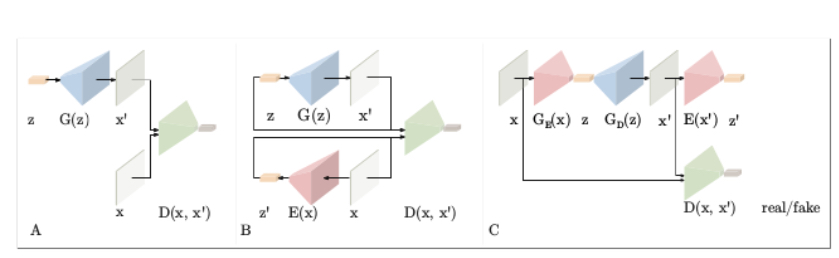
\includegraphics[height=5.5cm,width=12cm]{Report2-figure/image-20191001145242390.png}
  \caption{GAN BiGAN GANomaly}
  \end{figure}
\end{itemize}



\end{document}